\documentclass[11pt]{article}
\usepackage[margin=0.7in]{geometry}
\usepackage{multirow}
\usepackage {graphicx}
\usepackage[utf8x]{inputenc} % указать кодировку русского текста
\usepackage[russian]{babel} % указать, что язык текста - русский
\usepackage{fancyhdr}
\pagestyle{fancy}
\usepackage{graphicx}
\graphicspath{{pictures/}}
\DeclareGraphicsExtensions{.pdf,.png,.jpg}
\begin{document}
\begin{titlepage}
\begin{center}
\large\textbf{Московский Физико-Технический Институт}\\
\large\textbf{(государственный университет)}
\vfill
\huge\textbf{ Работа 3.1.3}\\
\huge\textbf{Измерение магнитного поля Земли}\\
\vfill
\large Факультет электроники, фотоники и молекулярной физики\\
\end{center}
\end{titlepage}
\fancyhead[L] {Работа 3.1.3}
\textbf{Цель работы}: исследовать свойства постоянных неодимовых магнитов; измерить с их помощью горизонтальную и вертикальную составляющие индукции магнитного поля Земли и магнитное наклонение.\\
\textbf{В работе используются}: неодимовые магниты, тонкая нить для изготовления крутильного маятника; медная проволка; элеткронные весы; секундомер; измеритель магнитной индукции; штангенциркуль; брусок, линейка и штатив из немагнитных материалов; набор гирь и разновесов.\\
\subsection*{Теория. Свойства точечного магнитного диполя}
Простейший магнитный диполь может быть образован витком с током или постоянным магнитом. По определению, магнитный момент $\overrightarrow{P_m}$ тонкого витка площадью $S$ с током $I$ равен
$$
\overrightarrow{P_m}=\frac{I}{c}\vec{S}=\frac{I}{c}S\vec{n},
$$
где $\vec{S}=S\vec{n}$ -- вектор площади контура. Если размеры контура с током или магнитной стрелки малы по сравнению расстоянием до диполя, то соответствующий магнитный диполь называют элементарным или точечным.\\
Магнитное поле точечного диполя определяется по формуле, аналогичной формуле для поля
элементарного электрического диполя:
$$
\vec{B}=\frac{3(\overrightarrow{P_m},\vec{r})\vec{r}}{r^5} - \frac{\overrightarrow{P_m}}{r^3}
$$ 
В магнитном поле с индукцией $B$
на точечный магнитный диполь 
действует механический
момент сил:
$$
\vec{M} = \overrightarrow{P_m}\times \vec{B}.
$$
Под действием вращающего момента $\vec{M}$ виток с током или постоянный магнит поворачивается
так, чтобы его магнитный момент выстроился вдоль вектора индукции магнитного поля. Это —
положение устойчивого равновесия: при отклонении от этого положения возникает механический
момент внешних сил, возвращающий диполь к положению равновесия. В положении, когда $\overrightarrow{P_m}$ и $\vec{B}$
параллельны, но направлены противоположно друг другу, также имеет место равновесие ($M$ = 0),
но такое равновесие неустойчиво: малейшее отклонение от этого положения приведёт к появлению
момента сил, стремящихся отклонить диполь ещё дальше от начального положения.\\
Магнитный диполь в магнитном поле обладает энергией:
$$
W = -(\overrightarrow{P_m},\vec{B})
$$
В неоднородном поле на точечный магнитный диполь, кроме момента сил, действует ещё и сила. Используя формулы для момента силы, силы и энергии, не сложно выяснить, как ведёт себя свободный магнитный диполь в неоднородном магнитном поле: он выстраивается вдоль силовых
линий магнитного поля и, кроме того, под действием результирующей силы, возникающей из-за неоднородности поля, втягивается в область более сильного магнитного поля, т.е. в область, где он
обладает меньшей энергией.\\
Зная магнитные моменты $P_1 = P_2 = P_m$ двух небольших постоянных магнитов, можно рассчитать силу их взаимодействия:
$$F = P_m \frac{\partial B}{\partial r}=-6\frac{P_m^2}{r^4}. $$
\subsection*{Экспериментальная установка. Неодимовые магнитные шары}
В настоящей работе используются неодимовые магниты шарообразной формы.
Для нас важно то, что:\\
1) шары намагничены однородно;\\
2) вещество, из которого изготовлены магниты, является магнитожёстким материалом.\\
Полный магнитный момент $\overrightarrow{P_m}$
постоянного магнита определяется намагниченностью $\overrightarrow{p_m}$
вещества, из которого он изготовлен. По определению, намагниченность – это магнитный момент единицы объёма. Для однородно намагниченного шара намагниченность равна:
$$
\overrightarrow{p_m}=\frac{\overrightarrow{P_m}}{V}.
$$
Намагниченность — важная характеристика вещества постоянных магнитов, определяющая, в
частности, величину остаточной магнитной индукции $B_r = 4\pi p_m$. Индукция магнитного поля $\overrightarrow{B_p}$
на полюсах однородно намагниченного шара связана с величиной намагниченности и остаточной магнитной индукцией формулами
$$
\overrightarrow{B_p}=\frac{8\pi}{3}\overrightarrow{p_m}=\frac{2}{3}\overrightarrow{B_r}.
$$
\section*{Описание работы}
\subsection*{Определение величины магнитного момента магнитных шариков}
\paragraph*{Метод А.}
Величину магнитного момента одинаковых шариков
можно рассчитать, зная их массу $m$ и определив максимальное расстояние $r_{max}$, на котором они ещё удерживают друг
друга в поле тяжести. При максимальном расстоянии сила тяжести шариков равна силе их магнитного притяжения:
\begin{center}
$\frac{6P_m^2}{r_{max}^4}=mg\Rightarrow$ \fbox{$P_m = \sqrt{\frac{mgr_{max}^4}{6}}$}
\end{center}
\paragraph*{Метод Б.}
Если сила сцепления двух одинаковых шаров диаметром $d$ c магнитными моментами $P_m$ равна:
$$
F_0 = \frac{6P_m^2}{d^4}
$$
то минимальный вес цепочки, при которой она оторвётся от верхнего шарика равен: $F \approx 1.08 F_0$. Тогда\\
\begin{center}
\fbox{$P_m = \sqrt{\frac{Fd^4}{6.48}}$}
\end{center}
\subsection*{Определение величины магнитного поля Земли}
\paragraph*{Горизонтальная составляющая.}
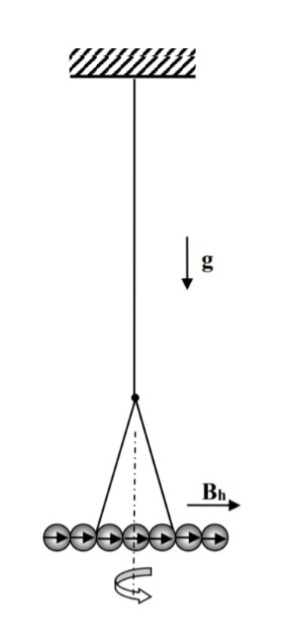
\includegraphics[width = 3cm]{g2}\\
Магнитная <<стрелка>> образована из $n$ сцепленных друг с другом противоположными полюсами шариков и с помощью $\Lambda$-образного подвеса подвешена в горизонтальном положении. При отклонении «стрелки» на угол $\theta$ от равновесного положения в горизонтальной плоскости возникают крутильные колебания вокруг вертикальной оси, проходящей через середину стрелки. При малых амплитудах уравнение колебаний
стрелки имеет вид:
$$
I_n \frac{d^2 \theta}{dt^2} + P_0 B_h \theta = 0,
$$ 
где $P_0$ -- магнитный момент стрелки, $B_h$ -- горизонтальная составляющая магнитного поля Земли, $I_n \approx \frac{1}{12}n^3 m d^3$, тогда период колебаний $T = kn$, где $k = \pi \sqrt{\frac{md^2}{3P_m B_h}}$. Измеряя зависимость $T=T(n)$, находится $B_h$:
\begin{center}
\fbox{$B_h = \frac{\pi^2 m d^2}{3k^2P_m}$}
\end{center}

\paragraph*{Вертикальная составляющая.} 
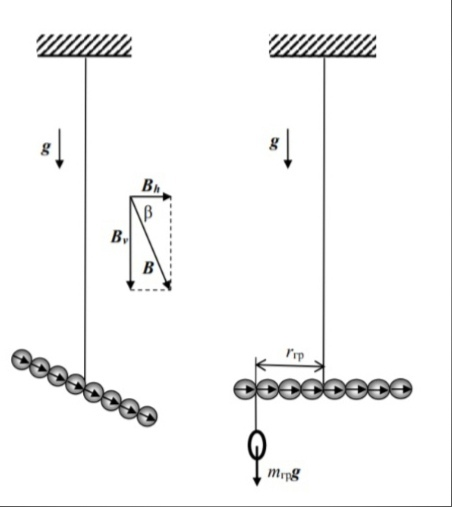
\includegraphics[width = 5cm]{g3}\\
Магнитная «стрелка», составленная из чётного числа
шариков и подвешенная на тонкой нити за середину, расположится не горизонтально, а под некоторым, отличным от нуля, углом к горизонту. Это связано с тем, что вектор $\vec{B}$ индукции магнитного поля Земли в общем случае не горизонтален, а образует с горизонтом
угол $\beta$, зависящим от географической широты $\varphi$
места, где проводится опыт. Величина угла $\beta$
называется магнитным наклонением.\\
С помощью небольшого дополнительного грузика «стрелку» можно «выровнять». Момент $M$ силы тяжести уравновешивающего груза пропорционален числу $n$ шариков, образующих магнитную «стрелку» $M(n) = An, A=P_m B_v$, то есть
\begin{center}
\fbox{$B_v = \frac{A}{P_m}$}
\end{center}
\section*{Ход работы}
\section*{1. Определение магнитного момента, намагниченности и остаточной магнитной индукции вещества магнитных шариков.}
1) Измерим диаметр и массу шариков в разном количестве, а потом усредним полученные результаты:\\
\\
Измерения диаметра проводились с помощью штангенциркуля\\
\\
\begin{tabular}{|l|l|l|l|l|l|l|l|l|l|l|}
\hline
$\sigma_{d}=0.1mm$&1&2&3&4&5&6&7&8&9&10\\
\hline
mm&5&5&5&5&5&5&5&5&5&5\\
\hline
\end{tabular}
\\
\\
Таким образом, \fbox{$d_{middle} = 5,0 \pm 0,1 \;mm$}\\
Измерение веса:\\
\\
\begin{tabular}{|l|l|l|}
\hline
$\sigma=0,001$ г.&Бумажки: 107,649 г. &Бумажки: 44,585 г.\\
\hline
10 шт& 112,456 г. & 49,433 г.\\
\hline
10 шт без бумажки & 4,807 г. & 4,848\\
\hline
20 шт& 117,259 г. & 54,242 г.\\
\hline
20 шт без бумажки & 9,61 г. & 9,657 г.\\
\hline 
30 шт & 122,107 г. & 59,045 г.\\
\hline
30 шт без бумажки & 14,458 г. & 14,46 г.\\
\hline
\end{tabular}
\\
\\
Тогда средний вес шарика:\\
$m_{middle} = \frac{4,807 + 4,848 + 9,61 + 9,657 + 14,458 + 14,46}{20 + 40 + 60} = \frac{57,84}{120} \approx 0,482$ г.\\
Таким образом, \fbox{$m_{middle} = 0,482 \pm 0,001 \; g$}\\
\\
2) Измерим индукцию $B_{p}$ на полюсах шарика с помощбю магнитометра:\\
Среднее значение, которое мы получили с помощью магнитометра: \fbox{$295,0 \pm 0,1 mT$}\\
3) Проложим между двумя магнитными шариками брусок из немагнитного материала. Подкладывая между бруском и верхним магнитиком листы бумаги, определим, на каком максимальном расстоянии $r_{max}$ шарики удерживают друг друга в поле тяжести Земли.\\
Грубо (подкладывали деревянные линейки толщиной 2 мм): $r_{max} = 16 \pm 2$ мм.\\
Точнее (подкладывали линейки и листы): $r_{max} = 16,8 \pm 0,1$ мм.\\
Тогда итоговый результат: \fbox{$r_{max} = 16,8 \pm 0,1\; mm$} \\
\\
4) Рассчитаем величину магнитного момента магнитика $\mu$:\\
$\mu = \sqrt{\frac{mg(r_{max}^4}{6}}$ (СГС)\\
$\mu = \sqrt{\frac{0,482g\times 9,8 сm/c^2 \times (1,68+0,5)^4 mm}{6}} \approx 42,2$ (СГС)\\
Рассчитаем погрешность:\\
$(\frac{\sigma_{\mu}}{\mu})^2 = 0,25(\frac{\sigma_{m}}{m})^2 + 0,25(\frac{\sigma_{g}}{g})^2 + 4(\frac{\sigma_{\sigma_{r_{max}}}}{r_{max}})^2$\\
$(\frac{\sigma_{\mu}}{\mu})^2 = 0,25(\frac{0,001}{0,482})^2 + 0,25(\frac{0,1}{9,8})^2 + 4(\frac{0,1}{16,8})^2 \approx 0,000168$\\
$\sigma_{\mu} \approx 0,5$\\
Тогда в итоге: \fbox{$\mu_{1} = 42,2 \pm 0,5 \;erg/gs$}\\
5) Используя дополнительные шарики, составим цепочку из 20-30 шариков, подбирая такой минимальный вес системы цепочки с гирей, при котором она отрывается от верхнего шарика.\\
Вес оторванной цепочки: \fbox{$m = 190,480 \pm 0,001 g$}\\
6) Рассчитаем силу сцепления двух шаров и по ней определим магнитный момент шарика $\mu$:\\
$F \approx 1,08F_{0}$\\
$F_{0} = \frac{3\mu^2}{8R^4}$\\
$\mu = \sqrt{\frac{8mgR^4}{3,24}}$\\
$\mu = \sqrt{\frac{8 \times 190,48g \times 980 cm/s^2 \times 0,25^4 (cm)^4}{3,24}} \approx 42,43 \approx 42,4$\\
Рассчитаем погрешность:\\
$(\frac{\sigma_{\mu}}{\mu})^2 = 0,25(\frac{\sigma_{m}}{m})^2 + 0,25(\frac{\sigma_{g}}{g})^2 + 4(\frac{\sigma_{R}}{R})^2$\\
$(\frac{\sigma_{\mu}}{\mu})^2 = 0,25(\frac{0,001}{190,48})^2 + 0,25(\frac{0,1}{9,8})^2 + 4(\frac{0,1}{2,5})^2 \approx 0,0064$\\
$\sigma_{\mu} \approx 3,4$\\
Таким образом, \fbox{$\mu_{2} = 42,4 \pm 3,4\; erg/gs$}\\
Относительная огрешность измерения магнитного момента в методе А составляет около 1$\%$, в то время как в методе Б - около 8$\%$. Результаты двух методов сходятся с хорошей точностью, однако в дальнейшем будем всё-таки использовать результаты метода А, как метода с наименьшей относительной погрешностью.\\
6) Рассчитаем величину намагниченности материала шариков М и остаточную индукцию магнитного поля $B_{r}$.\\
Для однородно намагниченного шара: $\mu = MV$\\
Поэтому $M = \frac{3\mu}{4\pi R^3}$\\
$M = \frac{3 \times 42,2}{4 \times 3,14 \times 0,25^4} \approx 2580, 4 \approx 2580$\\
Рассчитаем погрешность:\\
$(\frac{\sigma_{M}}{M})^2 = (\frac{\sigma_{\mu}}{\mu})^2 + (\frac{\sigma_{\pi}}{\pi})^2 + 9(\frac{\sigma_{R}}{R})^2$\\
$(\frac{\sigma_{M}}{M})^2 = (\frac{0,5}{42,2})^2 + (\frac{0,01}{3,14})^2 + 9(\frac{0,1}{2,5})^2 \approx 0,0145$\\
$\sigma_{M} \approx 311$\\
Таким образом: \fbox{$M = 2580 \pm 311 \; erg/(gs\times cm^3)$}\\
Теоретически: $B_r = 4\pi M $ (СГС)\\
$B_{r} = 4\times 3,14 \times 2580 \approx 32405 gs$
$B_{p} = B_{0} = \frac{2}{3}B_{r}$\\
$B_{p} \approx 21603 gs$\\
$\frac{\sigma_{B_{r}}}{B_r} = \frac{\sigma_{B_{p}}}{B_p} \approx \frac{\sigma_{M}}{M}$, поэтому\\
Индукция внутри и на полюсах шара: $B_{p} (Tesla) = B_{p}(gs) \times 0,0001 \approx 2,16 T$\\
 \fbox{$B_{p} = 2,16 \pm 0,26 \;T$}\\
 В то время как индукция, измеренная магнитометром, составляет примерно 0,3 Т. Думаю, что такие расхождения связаны с неточным способом измерения индукции: значения скачут сильно при попытке найти полюс, поэтому не всегда возможно их отследить.\\
 \section*{2. Определение горизонтальной составляющей магнитного поля Земли.}
 1) Соберем крутильный маятник из 12 магнитных шариков и подвесим его на немагнитный штатив. Используя лямбда-образный подвес, установим "магнитную" стрелку в горизонтальное положение.\\
 2) Возбудим крутильные колебания маятника вокруг вертикальной оси и определим их период, заранее убедившись в том, что упругость нити при расчёте периода колебаний можно не учитывать.\\
 3) Исследуем зависимость периода T крутильных колебаний "стрелки" от количества магнитных шариков n, составляющих "стрелку". 
 В данной таблице записано среднее значение периода по пяти измерениям для каждого количества шариков n.\\
 \\
 \begin{tabular}{|l|l|l|l|l|l|l|l|l|l|l|}
 \hline
 n&3&4&5&6&7&8&9&10&11&12\\
 \hline
 $<T>,\; c,\; \sigma_{T} = 0,4 \;c$&0,85&2,45&2,55&2,78&2,86&5,3&5,5&5,66&6,23&7,44\\
 \hline
 \end{tabular}\\
 \\
 Аппроксимируем полученную экспериментальную кривую по МНК:\\
 $ y = kx + b $\\
$ b = <y> - k<x> $\\
$ k = \frac{<yx> - <y><x>}{<x^2> - (<x>)^2} $\\
$ \sigma_{k} = \sqrt{\frac{1}{n-1}(\frac{<y^2> - (<y>)^2}{<x^2> - (<x>)^2} - k^2)} $\\
$ \sigma_{b} = \sigma_{k}\sqrt{<x^2> - (<x>)^2} $\\
$ k = \frac{36,811 - 7,5\times 4,162}{64,5 - 56,25} \approx 0,678 $\\
$ \sigma_{k} = \sqrt{\frac{1}{9}(\frac{21,368 - 4,162^2}{64,5 - 56,25} - 0,678^2)} \approx 0,06 $\\
$ b = 4,162 - 0,678\times7,5 \approx -0,923 $\\
$ \sigma_{b} = \sigma_{k}\sqrt{8,25}\approx 0,17 $\\
Таким образом, итоговая аппроксимирующая прямая: \fbox{$ y = 0,678x - 0,923$}\\
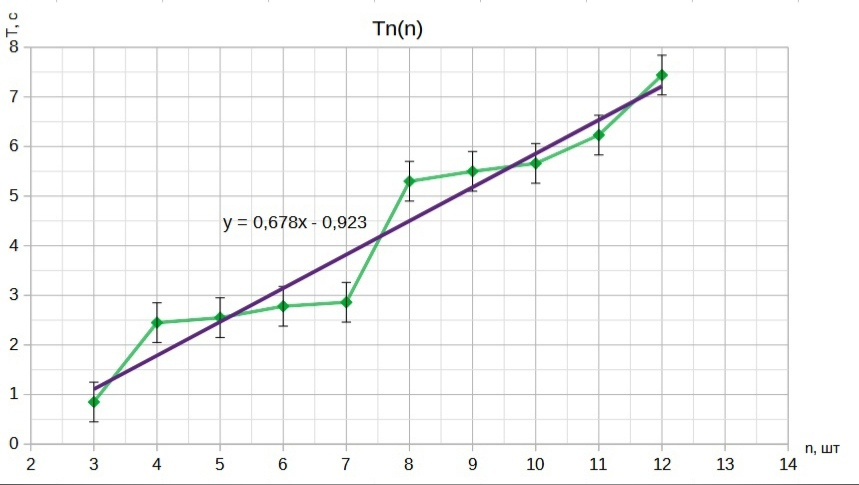
\includegraphics[width = 19cm]{g1}\\
\\
Горизонтальная составляющая поля равна: $B_h = \frac{\pi^2 m d^2}{3k^2P_m}$\\
$B_{h} = \frac{9,8596 \times 0,482 \times 0,5^2}{3 \times 0,678^2 \times 42,2} \approx 0,11$ Гс\\ 
$(\frac{\sigma_{B_h}}{B_h})^2 = 4(\frac{\sigma_{\pi}}{\pi})^2 + (\frac{\sigma_{m}}{m})^2 + 4(\frac{\sigma_{d}}{d})^2 + 4(\frac{\sigma_{k}}{k})^2 + (\frac{\sigma_{\mu}}{\mu})^2 = 4(\frac{0,01}{3,14})^2 + (\frac{0,001}{0,482})^2 + 4(\frac{0,1}{5})^2 + 4(\frac{0,06}{0,678})^2 + (\frac{0,5}{42,2})^2 \approx 0,00174$\\
$\sigma_{B_h} \approx 0,005$\\
Тогда горизонтальная составляющая: \fbox{$B_h = 0,110 \pm 0,005 \; gs$}\\
Такое маленькое значение получилось из-за достаточно большого коэффициента наклона графика, что в свою очередь связано с неточностью измерения периода колебаний (всё фиксировалось на глаз).
 \section*{3. Определение вертикальной составляющей магнитного поля Земли.}
 1) Изготовим магнитную "стрелку" из n = 12 шариков и подвесим её за середину с поомщью нити на штативе.\\
 2) Определим механический момент сил, действующий со стороны магнитного поля Земли на горизонтально расположенную магнитную "стрелку". С помощью весов измерим массу уравновешивающего груза $m_{gr}$. Из условий рассчитаем механический момент сил, действующих на горизонтальную "стрелку" со стороны поля Земли. Измерения проведем для четных значений n = 4,6,8,10,12.\\
 \\
 \begin{tabular}{|l|l|l|l|l|l|}
 \hline
 n&4&6&8&10&12\\
 \hline
 $r_{gr}, d$&1&2&4&5&4\\
 \hline
 $m_{gr}$, г.&0,130&0,103&0,103&0,103&0,170\\
 \hline
 \end{tabular}\\
 \\
 $M_{n} = m_{gr}gr_{gr} = n \mu B_{v}$\\
 \begin{tabular}{|l|l|l|l|l|l|}
 \hline
 n&4&6&8&10&12\\
 \hline
 $M_n$&63,7&100,94&201,88&254,8&333,2\\
 \hline
 \end{tabular}\\
 \\
Аппроксимируем полученную экспериментальную кривую по МНК:\\
 $ y = kx + b $\\
$ b = <y> - k<x> $\\
$ k = \frac{<yx> - <y><x>}{<x^2> - (<x>)^2} $\\
$ \sigma_{k} = \sqrt{\frac{1}{n-1}(\frac{<y^2> - (<y>)^2}{<x^2> - (<x>)^2} - k^2)} $\\
$ \sigma_{b} = \sigma_{k}\sqrt{<x^2> - (<x>)^2} $\\
$ k = \frac{1804,376 - 1527,232}{72 - 64} \approx 34,6 $\\
$ \sigma_{k} = \sqrt{\frac{1}{4}(\frac{46189,4776 - 36444,337}{72 - 64} - 34,6^2)} \approx 2,3 $\\
$ b = 190,904 - 34,6\times 8 = -85,9 $\\
$ \sigma_{b} = \sigma_{k}\sqrt{8}\approx 6,5 $\\
Таким образом, итоговая аппроксимирующая прямая: \fbox{$ y = 34,6x - 85,9$}\\
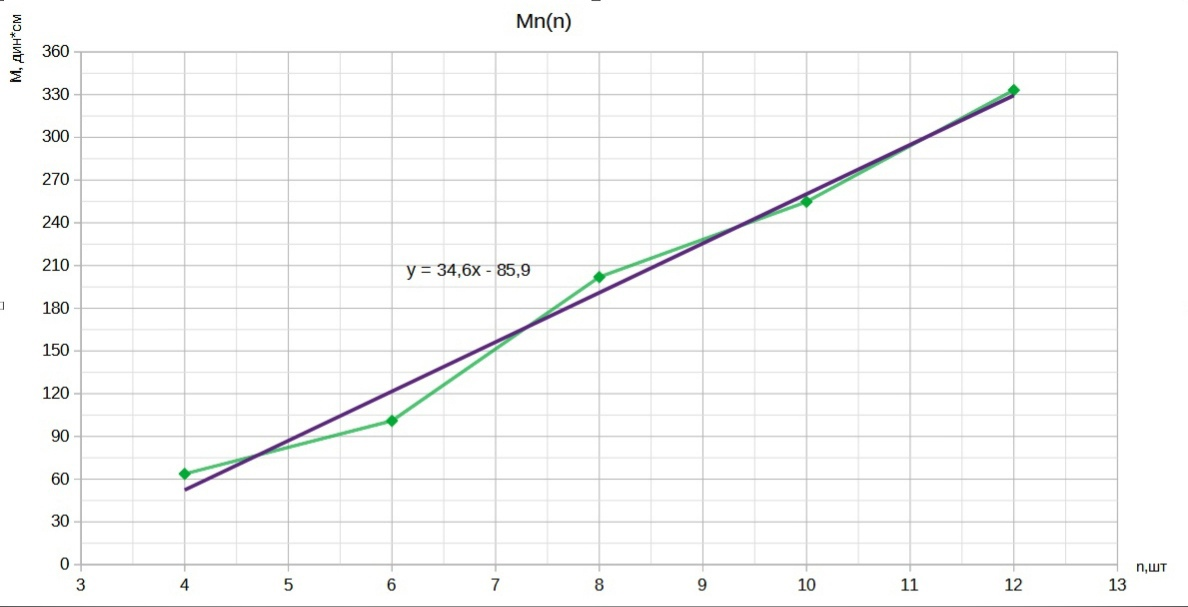
\includegraphics[width = 19.5cm]{g4}\\
\\
$B_{v} = \frac{M_n}{n\mu} = \frac{k}{\mu}$\\
$B_{v} = \frac{34,6}{42,2} \approx 0,82$ Гс\\
$(\frac{\sigma_{B_v}}{B_v})^2 = (\frac{\sigma_k}{k})^2 + (\frac{\sigma_{\mu}}{\mu})^2 = (\frac{2,3}{34,6})^2 + (\frac{0,5}{42,2})^2 \approx 0,00456 $\\
$\sigma_{B_v} \approx 0,05$ Гс\\
Тогда вертикальная составляющая: \fbox{$B_v = 0,82 \pm 0,05 \; gs$}\\
\section*{4. Определение полной составляющей магнитного поля Земли.}
$B = \sqrt{B_{v}^2 + B_{h}^2} = \sqrt{0,11^2 + 0,82^2} \approx 0,83$ Гс\\
$(\frac{\sigma_{B}}{B})^2 = (\frac{\sigma_{B_v}}{B_v})^2 + (\frac{\sigma_{B_h}}{B_h})^2 = (\frac{0,05}{0,82})^2 + (\frac{0,005}{0,110})^2 \approx 0,00578 $\\
$\sigma_{B} \approx 0,06$ Гс\\
Таким образом, \fbox{$B = 0,83 \pm 0,06 \; gs$}\\
Определим магнитное наклонение $\beta$:\\
$tg(\beta) = \frac{B_v}{B_h} = \frac{0,82}{0,11} \approx 7,45$\\
$\beta = arctg(7,45) \approx 82 $ градуса Цельсия
\section*{5. Вывод и сравнение данных}
Табличные значения для Московского региона находятся в диапазоне 0,60 - 0,65 Гс, поэтому полученные кспериментальные значения оказались приблизительно на 30$\%$ больше. 

\end{document}